\documentclass[UTF8]{article}

%--
\usepackage{ctex}
\usepackage{graphicx}
\usepackage[margin=1in]{geometry}

%--
\begin{document}
    
%--
{\flushleft \bf \Large 姓名:} 汪浩港

{\flushleft \bf \Large 学号:} MG1833067

{\flushleft \bf \Large 日期:} 2018.12.4

%=========================================================================
\section*{命名实体识别}
    
    
%=========================================================================
\section{任务描述}

NER(Named Entity Recognition,命名实体识别)又称作专名识别,是自然语言处理中常见的一项任务,使用的范围非常广。命名实体通常指的是文本中具有特别意义或者指代性非常强的实体,通常包括人名、地名、机构名、时间、专有名词等。NER系统就是从非结构化的文本中抽取出上述实体,并且可以按照业务需求识别出更多类别的实体,比如产品名称、型号、价格等。因此实体这个概念可以很广,只要是业务需要的特殊文本片段都可以称为实体。

本次任务就是从已经分好词的中文文本中识别出人名(PERSON)、地点(LOCATION)、时间(TIME)及机构名(ORGANIZATION)。



%=========================================================================
\section{技术路线}

\subsection{运行环境}
开发与测试系统:Ubuntu18.04

开发语言:Python3.6

硬件平台:Alienware-Area-51-R5(配置双1080Ti)

cuda版本:9.2

tensorflow版本:1.12


执行方法是只需运行NER目录下的run.sh脚本即可,预测结果是NER/results/test.prediction.txt。
\subsection{模型概述}
该模型基于BiLSTM-CRF[1]。 模型主要有三个组成部分:

\begin{itemize}
	\item \textbf{Word Representation}: 使用预训练的300维中文词向量,对于没有对应的预训练词向量的词,使用全零向量。我还将从字中提取一些含义。许多实体没有预先训练的词向量,对每个词的字也做编码后作为输入的一部分。
	\item \textbf{Contextual Word Representation}: 对于其上下文中的每个单词,需要获得有意义的表示,这里使用LSTM。
	\item \textbf{Decoding}: 从上一步中得到每一个词的向量,使用条件随机场(CRF)处理它来做出最终的预测。
\end{itemize}

模型框架如图1所示
\begin{center}
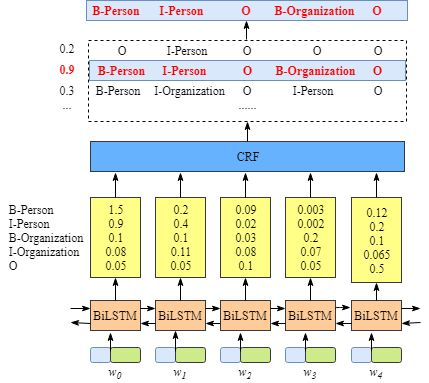
\includegraphics[scale=0.8]{BiLSTM-CRF.jpg} \\
图1 BiLSTM-CRF
\end{center}
%=========================================================================
\subsubsection{Word Representation}
对于每个单词,需要构建一个n维的向量(本次任务中n=400)。 我通过将预训练的词向量和从单字级别特征训练得到的向量联结起来得到它。在本次任务中,我将在单字级别使用双向LSTM,但也可以在单字或n-gram级别使用任何其他类型的递归神经网络甚至卷积神经网络,本次任务中并没有包含这些尝试。

对于一个词中的每个字,它都与一个$d_1$维向量相关联,在字embedding序列上训练双向LSTM并连接最终状态以获得$d_2$维向量。将词向量与这个向量连接后得到所需要的向量。

\subsubsection{Contextual Word Representation}
在词向量序列上训练双向LSTM后得到另一个词向量序列(两个隐藏状态的连接)。我使用每个时间步的隐藏状态而不仅仅是最终状态,将一个词向量序列作为输入,得到另一个词向量序列,它不但只包含词级别的信息,还能表达上下文,代码如下所示。
 \begin{verbatim}
 cell_fw = tf.contrib.rnn.LSTMCell(hidden_size)
 cell_bw = tf.contrib.rnn.LSTMCell(hidden_size)
 
 (output_fw, output_bw), _ = tf.nn.bidirectional_dynamic_rnn(cell_fw,
 cell_bw, word_embeddings, sequence_length=sequence_lengths,
 dtype=tf.float32)
 
 context_rep = tf.concat([output_fw, output_bw], axis=-1)
 \end{verbatim}
 \subsubsection{Decoding}
 现在,每一个词$w$和一个向量$h$相关联,使用全连接的神经网络得到一个向量,在其中,每个元素对应一个标签(tag)的分数。代码如下所示。
 ,还能表达上下文,代码如下所示。
 \begin{verbatim}
 W = tf.get_variable("W", shape=[2*self.config.hidden_size, self.config.ntags],
 dtype=tf.float32)
 
 b = tf.get_variable("b", shape=[self.config.ntags], dtype=tf.float32,
 initializer=tf.zeros_initializer())
 
 ntime_steps = tf.shape(context_rep)[1]
 context_rep_flat = tf.reshape(context_rep, [-1, 2*hidden_size])
 pred = tf.matmul(context_rep_flat, W) + b
 scores = tf.reshape(pred, [-1, ntime_steps, ntags])
 \end{verbatim}
 
 最后的工作就是解码这个向量,得到预测结果。我使用线性链条件随机场(linear-chain CRF)来做预测,给定一个词序列$w_1,\dots,w_m$,一个得分序列$s_1,\dots,s_m$,一个标签序列$y_1,\dots,y_m$,标签类别共有10种,CRF定义一个全局得分$C$,计算公式是$C(y_1,\dots,y_m)=b[y_1]+\sum_{t=1}^{m}s_t[y_t]+\sum_{t=1}^{m-1}T[y_t,y_t+1]+e[y_m]$。$T$是一个$10\times10$的转移矩阵,$e,b$分别是一个标签的开头和结尾对应的得分向量。
 
 之后需要找到有最好得分的标签序列并计算出所有标签序列的概率分布。前者应用动态规划解决,后者是将softmax应用于所有可能序列的分数,以获得给定序列标签的概率。
 \subsection{用到的数据}
 使用了第三方的预训练词向量,项目地址是https://github.com/Embedding/Chinese-Word-Vectors,我选择的词向量下载地址是https://pan.baidu.com/s/14JP1gD7hcmsWdSpTvA3vKA,它使用单词、单字和Ngram作为特征训练词向量。
 \section{遇到的问题及解决方案}
\begin{itemize}

	\item 如果要自己训练生成优质的词向量,需要大体积的词库和大量的计算资源,这个方案并不现实,改为使用网络上可以得到的预训练词向量。

\end{itemize}
\section{性能评价}

引入第三方优质词向量后性能有了极大的提升,最终正确率较高,使用训练25轮后的模型进行预测得到的结果评分为0.966441。该模型在GTX1080Ti上训练时间约为610s/epoch,10轮后可以得到较满意的模型,对测试集dev.txt进行预测后使用metrics.py评测后的结果如图2所示。
\begin{center}
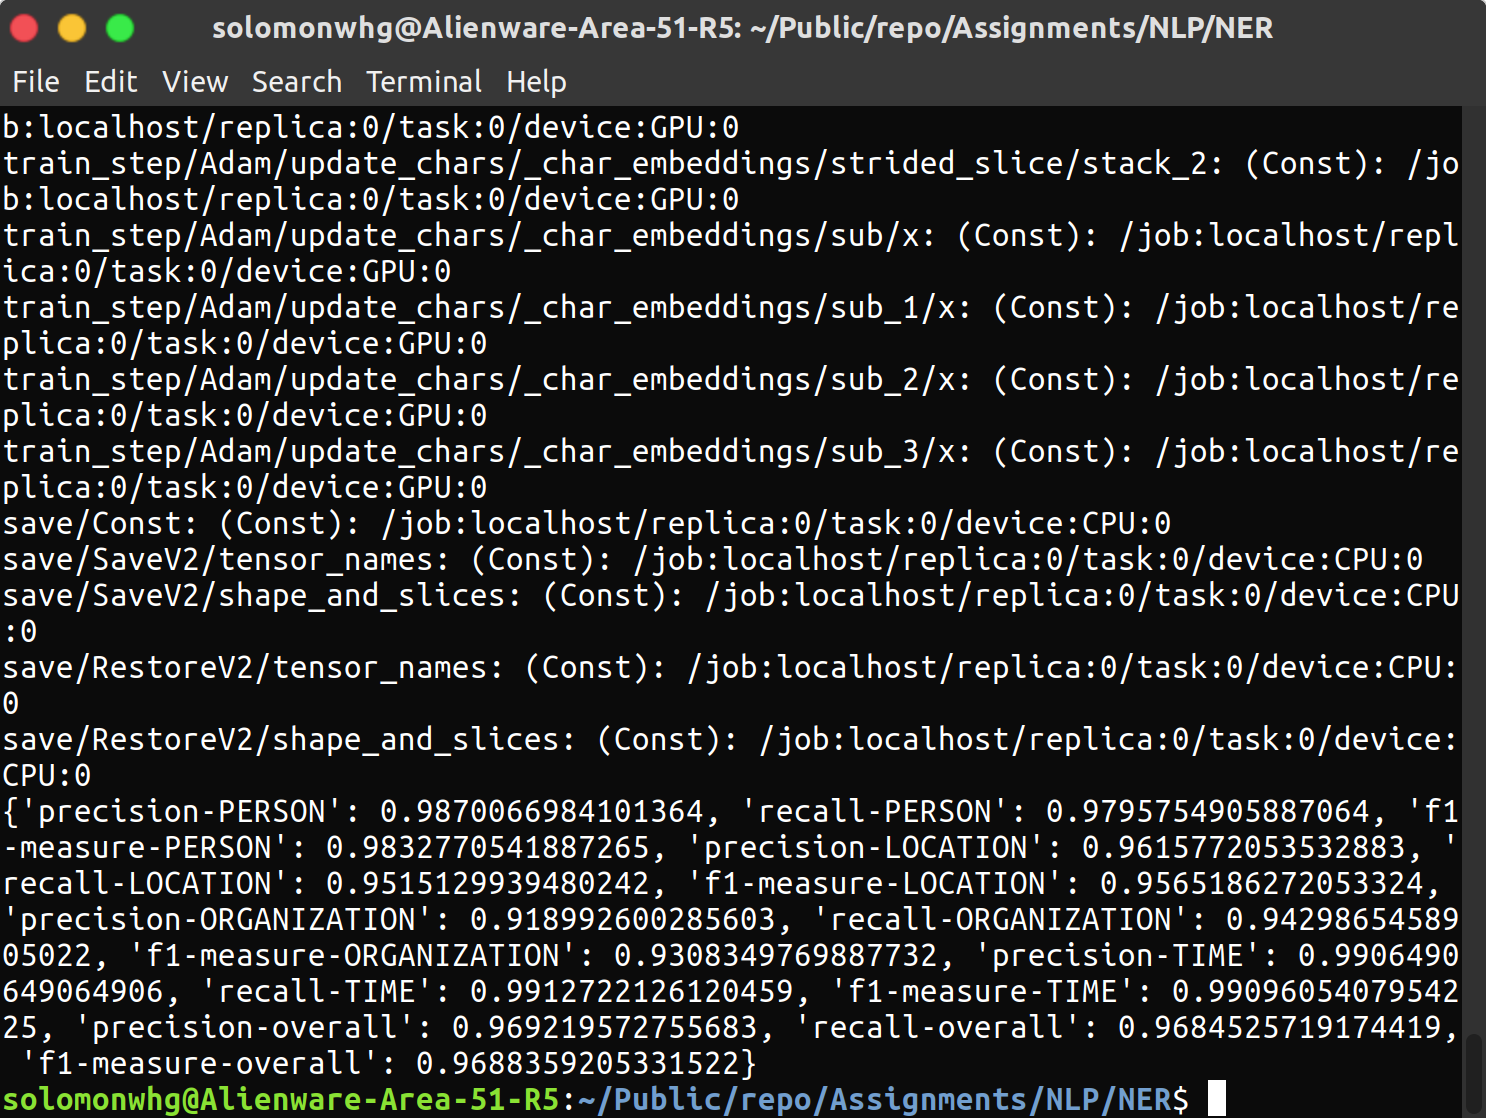
\includegraphics[scale=0.3]{运行截图.png} \\
	图2 测试集预测评分

\end{center}
\section*{reference}
[1] https://github.com/guillaumegenthial/sequence_tagging
\end{document}
